%#BIBTEX biber --bblencoding=utf8 -u -U --output_safechars main
%#!uplatex main.tex

\section{Preparation}

In this section, we introduce basic prerequisites to understand
Iterated Inversion System (IIS.)

In this paper, we mainly work on circle or sphere inversions.

\subsection{Kleinian Groups}

Kleinian groups is discrete sub-group of the M\"obius transformation
groups. Visualized images of Kleinian groups often have fractal structures.

\subsection{M\"obius Transformations and Inversions}

M\"obius transformations are defined in the extended complex plane,
$\hat{\mathbb{C}} = \mathbb{C} \cup \{\infty\}$ and expressed as linear
fractional transformation
$f(z)=\frac{az + b}{cz + d}$, where $a,~b,~c,~d,~z \in \hat{\mathbb{C}}$.
However, it is also known that we can construct them out of a finite
composition of inversions. For more details, see the introduction of \cite{mobius}.

M\"obius transformations are classified into three types as loxodromic,
parabolic, or elliptic.
Loxodromic transformations have two fixed points and are conjugate to
scaling by complex numbers except for scaling by unit complex numbers.
Those whose multiplier is a positive real number
are also called hyperbolic transformations.
Parabolic transformations have one fixed point and are conjugate to
parallel translations.
Elliptic transformations have two fixed points and are conjugate to rotations.

An inversion in a circle
is defined as $f(z) = \frac{r^2}{~\overline{z - c}~} + c$, where $c$ and
$r$ are center and radius of the circle.
Note that an inversion in a circle with infinite radius is the same as
a reflection over a line.
Also, sphere inversion can be derived from a similar equation, and an inversion
in a sphere with infinite radius is the same as
a reflection through a plane.

%% \subsection{Transformation Groups}
%% describe transformation groups, generator, snd word

\subsection{Basic Methods for Visualization}

\begin{figure}[htbp]
 \begin{minipage}[t]{0.5\hsize}
  \center
  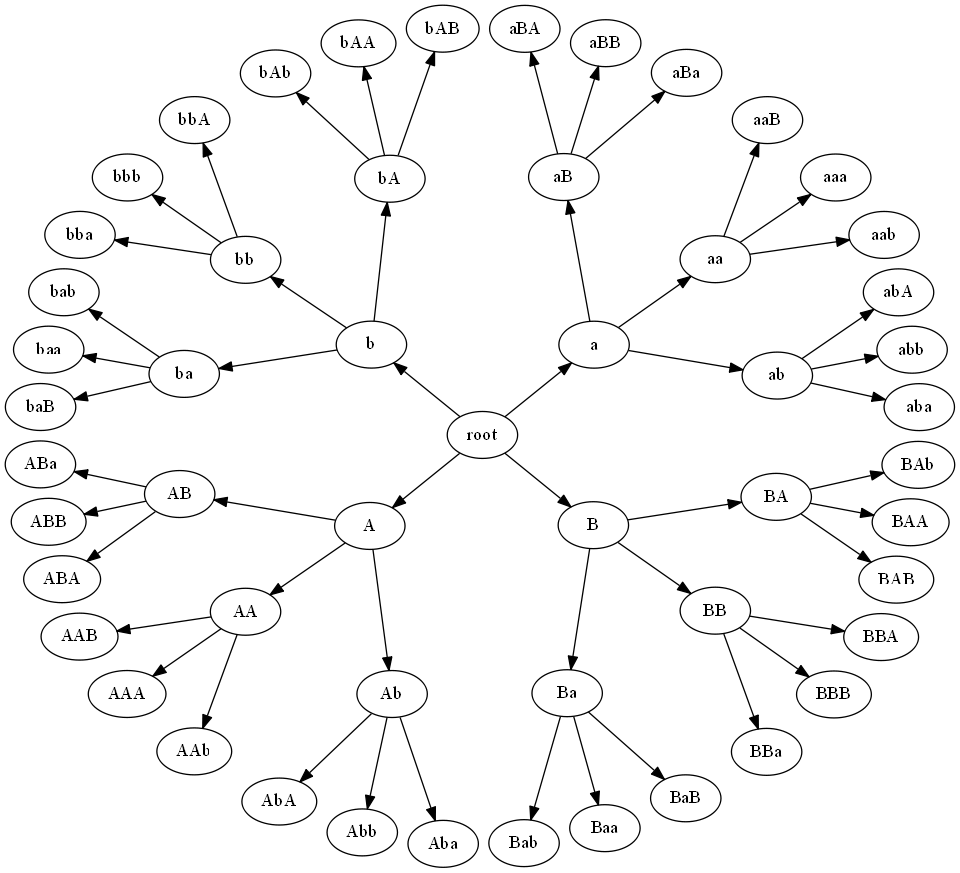
\includegraphics[height=1.35in, keepaspectratio]{img/cayleyGraph.png}
  \caption{\textit{Cayley Graph}}
  \label{fig:cayleyGraph}
  \hspace*{\fill}
 \end{minipage}
 \begin{minipage}[t]{0.5\hsize}
  \center
  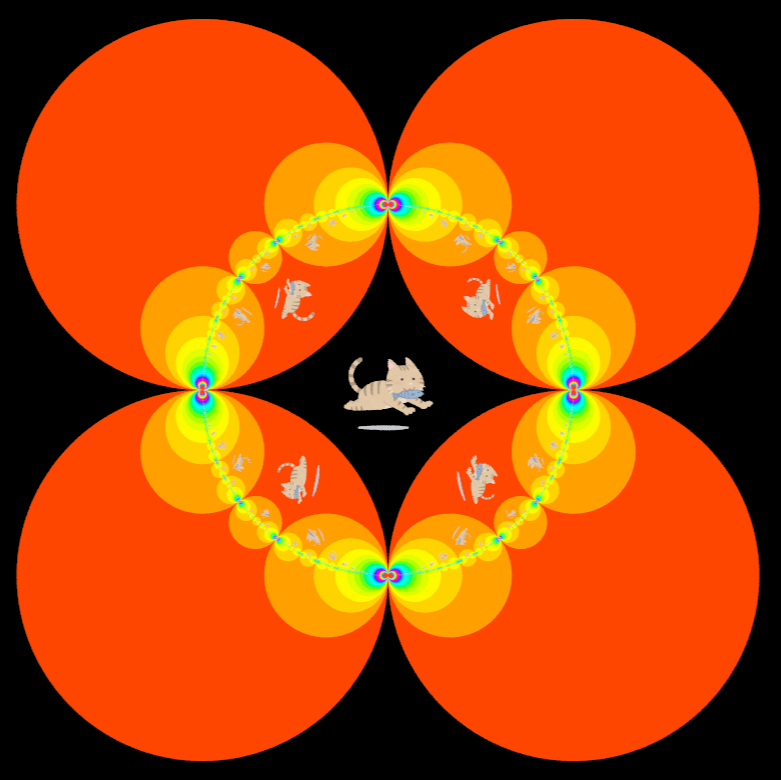
\includegraphics[height=1.35in, keepaspectratio]{img/preparation/basic/catOrbit.png}
  \caption{\textit{Orbit of the image}}
  \label{fig:orbitCat}
  \hspace*{\fill}
 \end{minipage}
\end{figure}

In this section, we introduce basic methods for visualizing Kleinian groups.
We consider \textit{cayley graph} of the Kleinian groups to enumerate elements
of the groups.
Figure \ref{fig:cayleyGraph} shows Cayley graph of Kleinian groups. The nodes of the graph
represent compositions of elements of the group.
According to the way of traversing, 
there are two types to visualize transformation groups.

Firstly, we can draw orbit of the group by traversing the cayley graph with
breadth first search.
We prepare fundamental tile, then we apply found words.
See Figure \ref{fig:orbitCat}.
Tiling of the first tile.
%% 種となる図に対し,探索で得られた語を作用させることで,その図の群によ
%% る軌道を描画することができる

Secondly, we can draw the limit set of the group by traversing the
cayley graph with depth first search.
We use fixed points of the groups.
we apply obtained word to the fixed points.
%% 極限集合はケーリーグラフの無限遠に存在している.そのため,固定点を用
%% いる.
%% 各固定点に探索で得られた語を作用させる

However, there are some faults in these methods.
For example, if we increase the number of generators,
It takes too much time to traverse the graph because of
combinatorial explosion.
Also, We have to traverse all of the graph
even though we don't need images outside of the screen.
This is the reason why we need other methods to visualize Kleinian
groups.
For more details about the methods, read Indra's Pearls \cite{MumfordSeriesWright200204}.

%% ここからは行列表現ではなく円や球の反転を用いてクライン群を描画する.
%% 円や球には幾何学的な直観が働くため,行列そのものを扱うよりは非常にわ
%% かりやすい.

\subsection{Iterated Inversion System (IIS)}

\begin{figure}[htbp]
 \begin{minipage}[t]{0.16\hsize}
  \center
  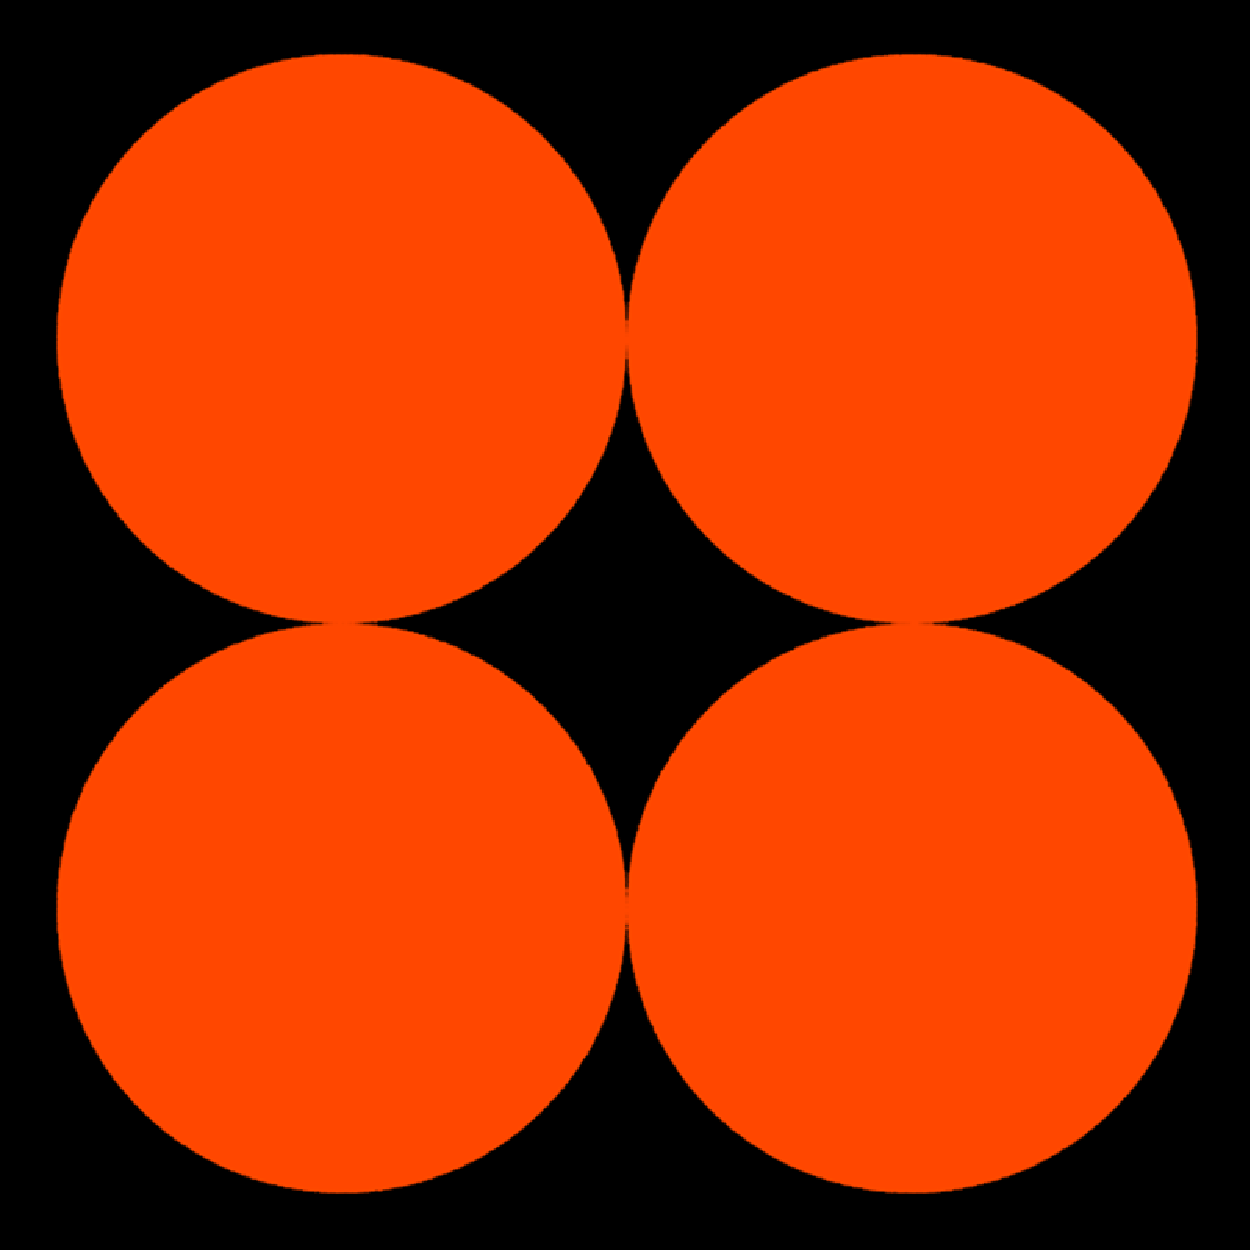
\includegraphics[width=1in, height=1in, keepaspectratio]{./img/preparation/orbit/level0c.pdf}
  \subcaption{}
  \label{fig:level0}
 \end{minipage}
 \begin{minipage}[t]{0.16\hsize}
  \center
  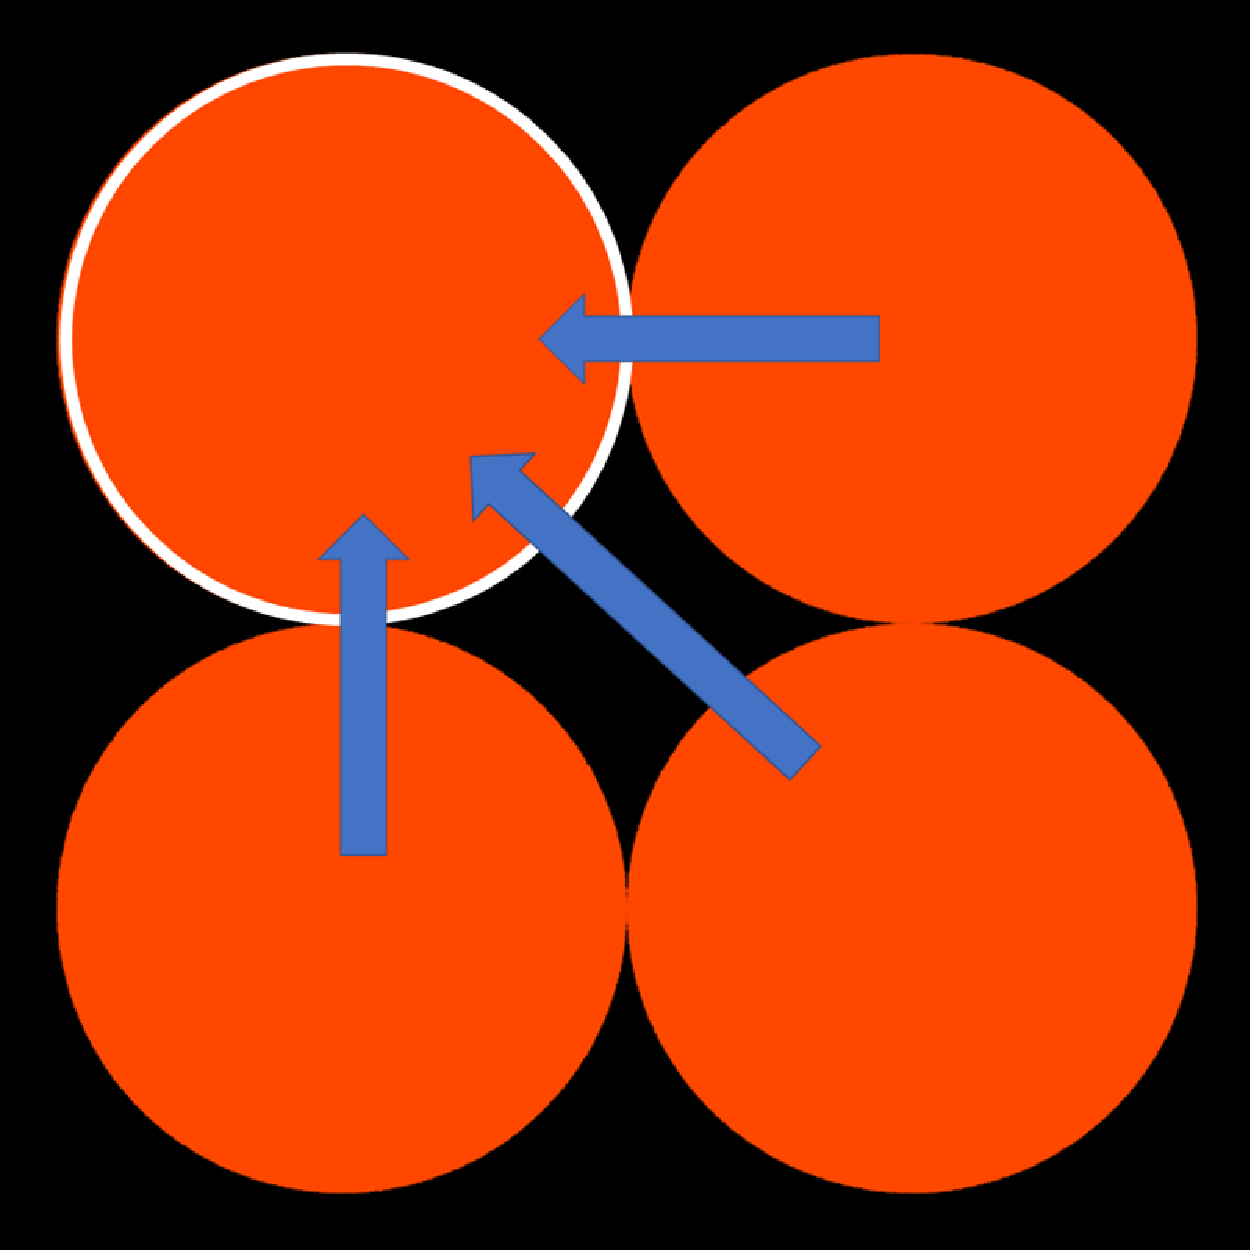
\includegraphics[width=1in, height=1in, keepaspectratio]{./img/preparation/orbit/level0invc.pdf}
  \subcaption{}
   \label{fig:level0inv}
 \end{minipage}
 \begin{minipage}[t]{0.16\hsize}
  \center
  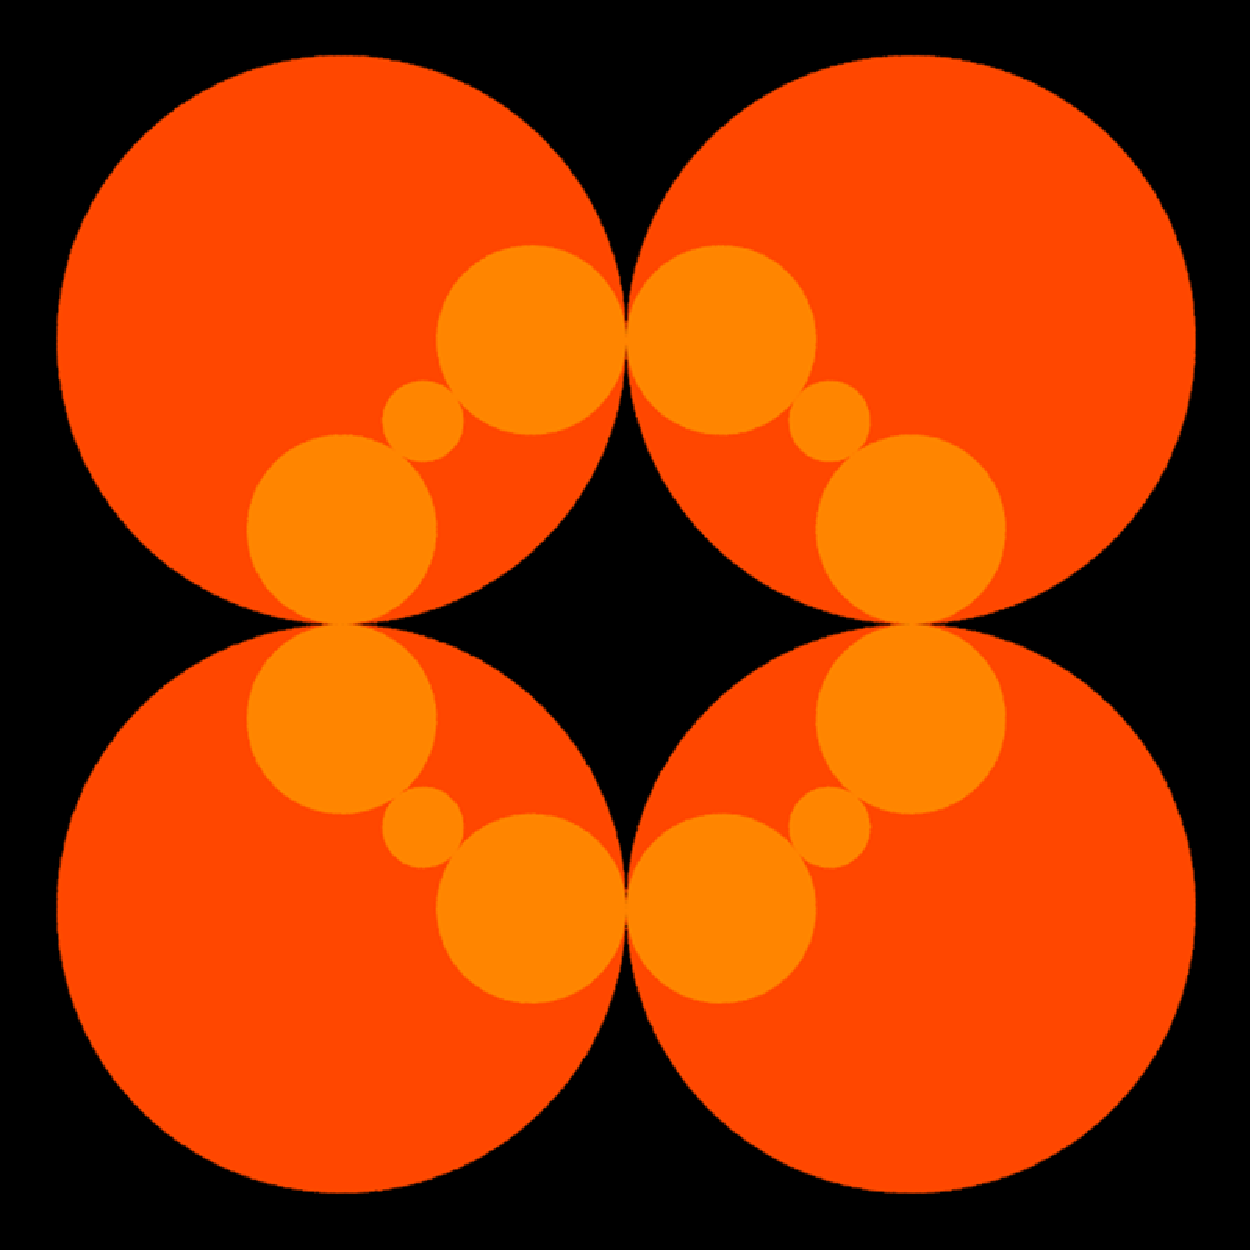
\includegraphics[width=1in, height=1in, keepaspectratio]{./img/preparation/orbit/level1c.pdf}
  \subcaption{}
   \label{fig:level1}
 \end{minipage}
 \begin{minipage}[t]{0.16\hsize}
  \center
  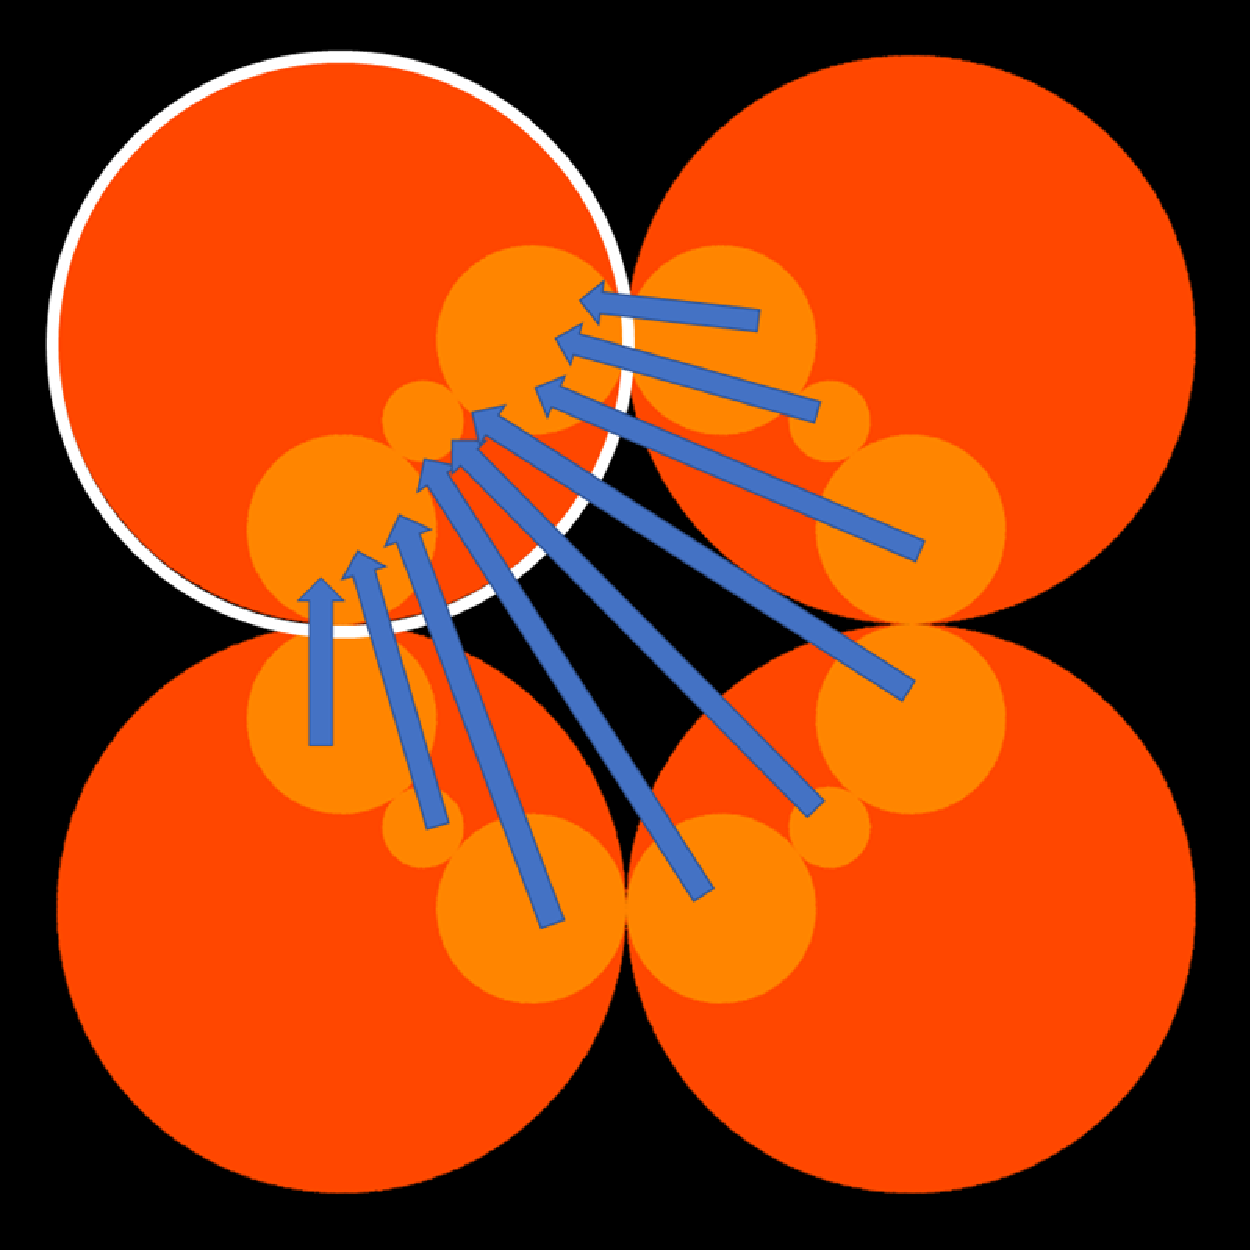
\includegraphics[width=1in, height=1in,
  keepaspectratio]{./img/preparation/orbit/level1invc.pdf}
  \subcaption{}
  \label{fig:level1inv}
 \end{minipage}
 \begin{minipage}[t]{0.16\hsize}
  \center
  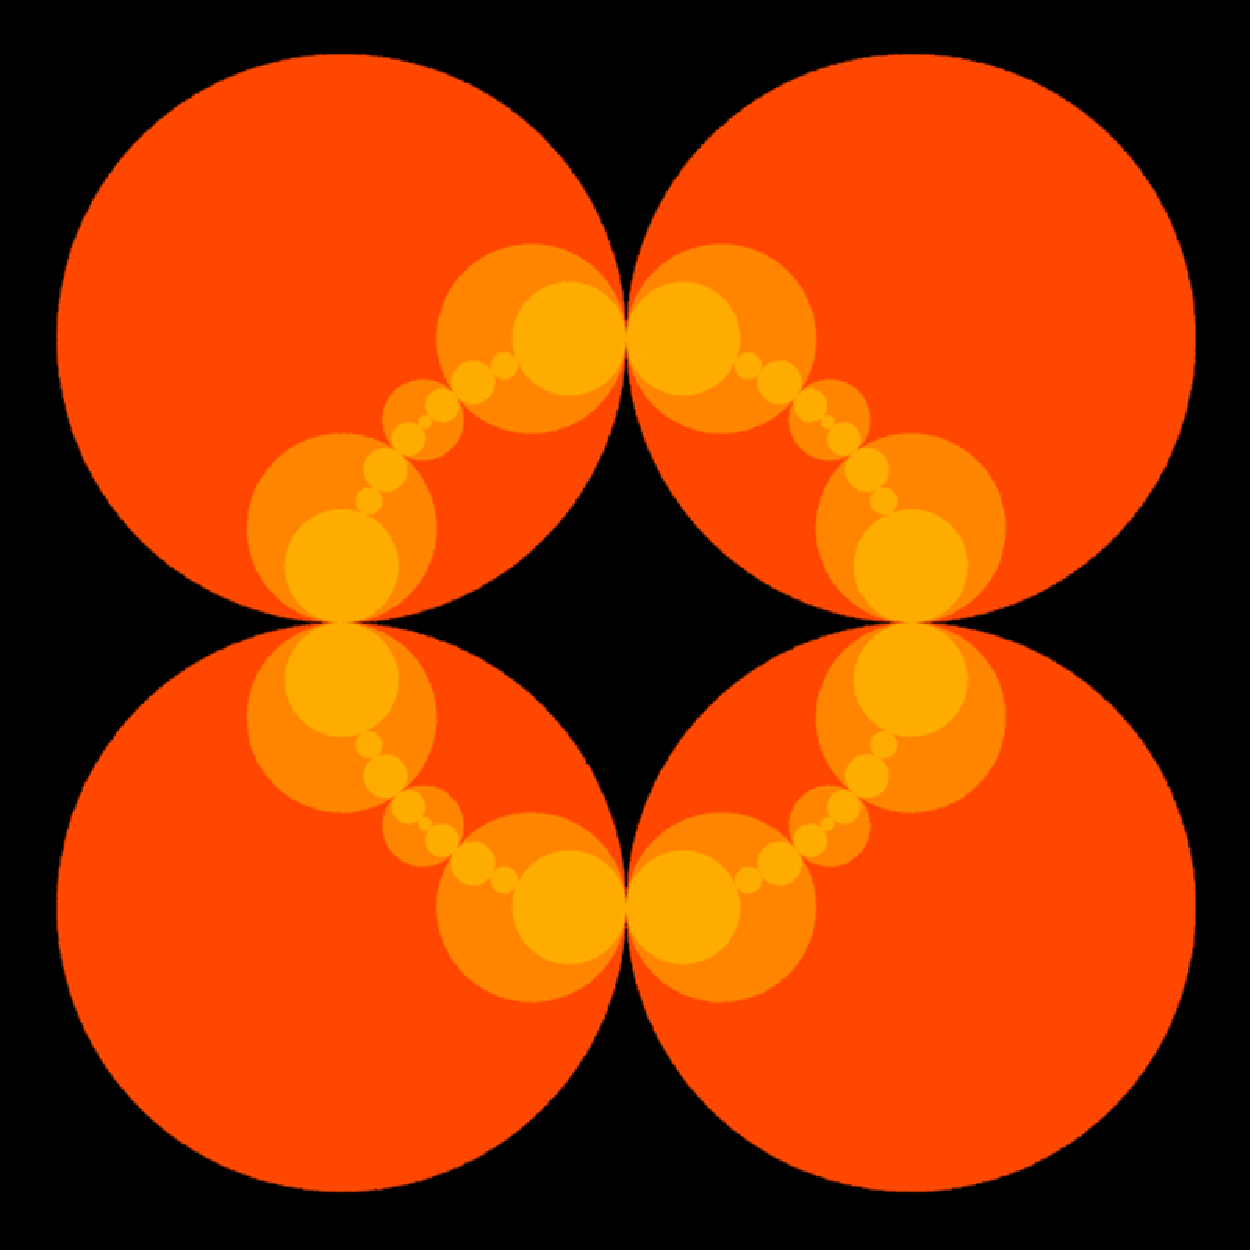
\includegraphics[width=1in, height=1in, keepaspectratio]{./img/preparation/orbit/level2c.pdf}
  \subcaption{}
  \label{fig:level2}
 \end{minipage}
 \begin{minipage}[t]{0.16\hsize}
  \center
  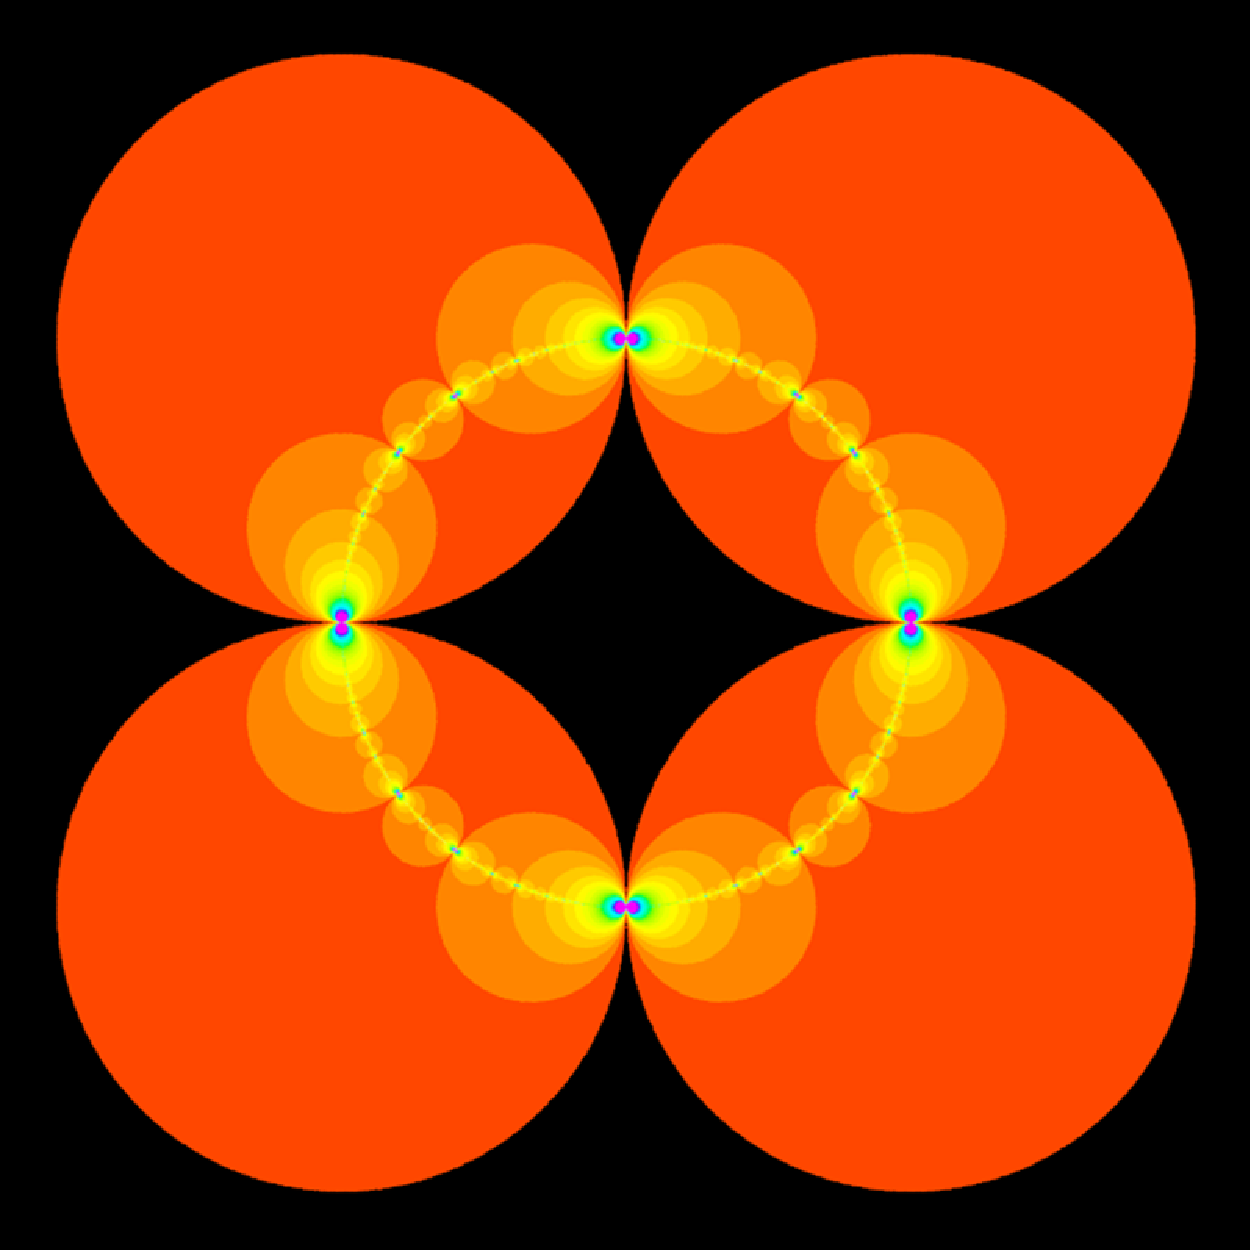
\includegraphics[width=1in, height=1in, keepaspectratio]{img/preparation/orbit/levelMaxc.pdf}
  \subcaption{}
  \label{fig:levelMax}
 \end{minipage}
 \caption{\textit{The process of rendering the orbit of Schottky disks}}
\end{figure}

To solve the problems we discussed in previous section,
we invent an efficient algorithm to visualize \textit{circle inversion
fractals} shown in Figure \ref{fig:levelMax}. 
The algorithm is called \textit{Iterated Inversion System (IIS.)}
It can visualize not only two dimensional fractals but
also three dimensional sphere inversion fractals.

The fractal in Figure \ref{fig:levelMax} shows the orbit of the first
four circles.
It is also Kleinian group composed of four circle inversions.
The process of generation of circle inversion fractals is
as follows.

\begin{enumerate}
 \item We need some disjoint disks to obtain circle inversion fractals.
       For example, we assume there are four orange disks as shown in
       Figure \ref{fig:level0}. We call orange disks \textit{initial
       disks} and their boundary \textit{initial circles}.
 \item First of all, we focus on the white circle in Figure
       \ref{fig:level0inv}. The inversion in the white circle moves the
       other three disks into the interior of the white circle.
 \item After we apply each inversion in the initial circle to the outer disks,
       we obtain twelve small disks. They are shown in Figure \ref{fig:level1}.
 \item Next, we invert the twelve small disks in the initial circles.
       The inversion in the white circle moves the outer nine small disks
       into the interior of the white circle as shown in Figure \ref{fig:level1inv}.
       Each inversion in the Schottky circle generates smaller disks, and we
       obtain Figure \ref{fig:level2}.
 \item We continue iterating these process, that is, we continue
       applying each inversion in the initial circle to resulting
       smaller disks.
       Finally, we get Figure \ref{fig:levelMax}.
\end{enumerate}

\subsubsection{Two Dimensional IIS}

\begin{figure}[htbp]
  \center
  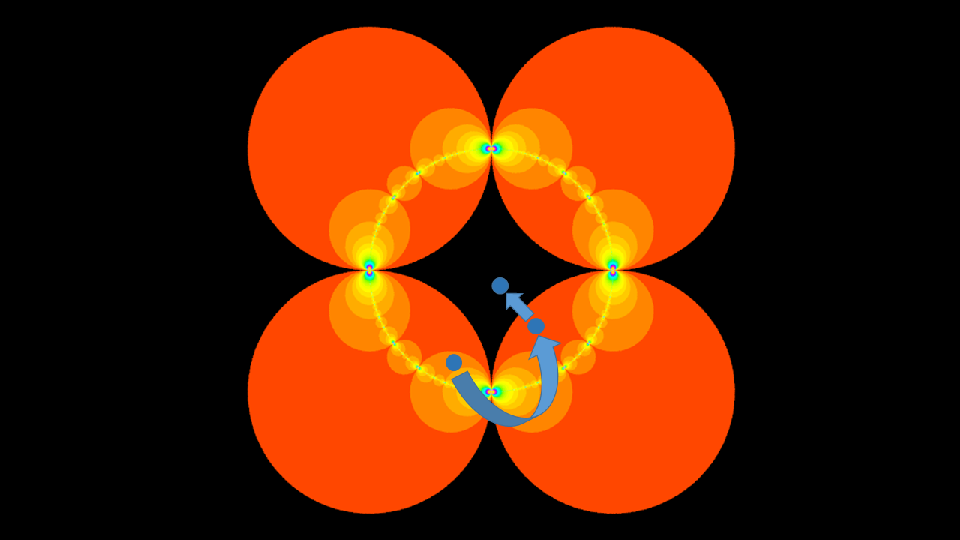
\includegraphics[height=1.35in, keepaspectratio]{img/preparation/orbIIS.png}
  \caption{\textit{Orbit of blue point by IIS}}
  \label{fig:iisOrbit}
 \hspace*{\fill}
\end{figure}

 \begin{algorithm}
  \caption{Iterated Inversion System (IIS)}
  \label{arg:iis2d}
  \begin{algorithmic}
   \REQUIRE count $= 0$ and coordinates $=$ position determined by
   pixel
   \FOR{$i=0$ to MAX\_INVERSION}
   \STATE inOutside $\leftarrow$ \TRUE
   \FOR{ each inversion $I$ in circles }
   \IF{The circle $I$ contains coordinates}
   \STATE coordinates $\leftarrow$ $I(\text{coordinates})$
   \STATE INCREMENT count
   \STATE inOutside $\leftarrow$ \FALSE
   \ENDIF
   \ENDFOR
   \IF {inOutside}
   \STATE BREAK for
   \ENDIF
   \ENDFOR
   \STATE RETURN count
  \end{algorithmic}
 \end{algorithm}

IIS computes the depth of the circles point by point.
Thus, we can use parallel processing.
The images in this paper are rendered using \textit{OpenGL Shading
Language (GLSL)}.
For two dimensional fractals, the algorithm of IIS is as follows.

IIS is applied to each point on the plane and computes nesting depth of
the disk which contains the point.
The process of the algorithm is as follows.
First of all, if the point is contained in initial disks, we invert the
point in the boundary circle of the disk.
We continue applying inversions until the transformed point is in the
out side of the initial circles.
Figure \ref{fig:iisOrbit} shows orbit of the blue point transformed by
iterations of inversions.
Pseudo-code is in Algorithm \ref{arg:iis2d}.

Furthermore, a point actually at the limit set never reaches the
outside. So, we have to determine the maximum number of iterations in
advance to prevent the algorithm from running indefinitely.
However, the points except for the limit set are guaranteed that they
are transformed to outside because inversions are involution.

\subsubsection{Three Dimensional Extension}

%% 二次元と同様に描画すると球が球の内側に連なってしまい,描画するのが難
%% しくなってしまう.例えばこれを描画するために, volume rendering という
%% 手法があるが,描画に時間がかかるうえ,得られる図もあまり面白くない.
%% そこで,二次元同様にもの(球)をおいてその軌道を描画するように変更した.

In the similar manner to two dimensional algorithm,
we extend the IIS to visualize three-dimensional kleinian groups.
We extend circle inversion to sphere inversion easily, and we
compute the nesting depth of the sphere voxel by voxel.

However, it is difficult to render nesting spheres efficiently, and
visualized images are not interesting.

We use \textit{ray tracing} to visualize three dimensional objects.
Ray tracing computes intersection between ray and objects algebraically.

as transparent spheres or volume rendering.
volume rendering using \textit{ray marching}.
This is not efficient algorithm, and resulting images are not interesting.

\begin{figure}[htbp]
 \begin{minipage}[t]{0.5\hsize}
  \center
  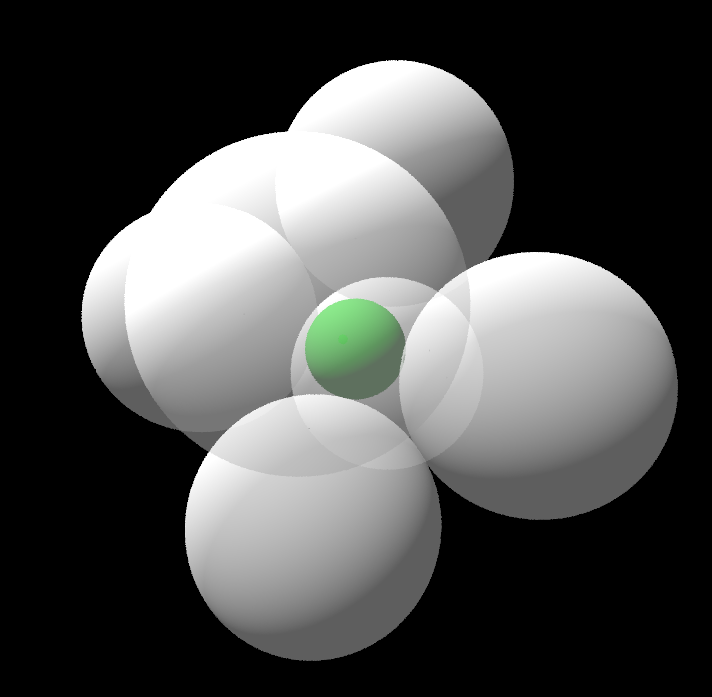
\includegraphics[height=1.35in, keepaspectratio]{img/preparation/3dExtension/3dKissingGenerator.png}
  \caption{\textit{Generator}}
  \label{fig:cayleyGraph}
  \hspace*{\fill}
 \end{minipage}
 \begin{minipage}[t]{0.5\hsize}
  \center
  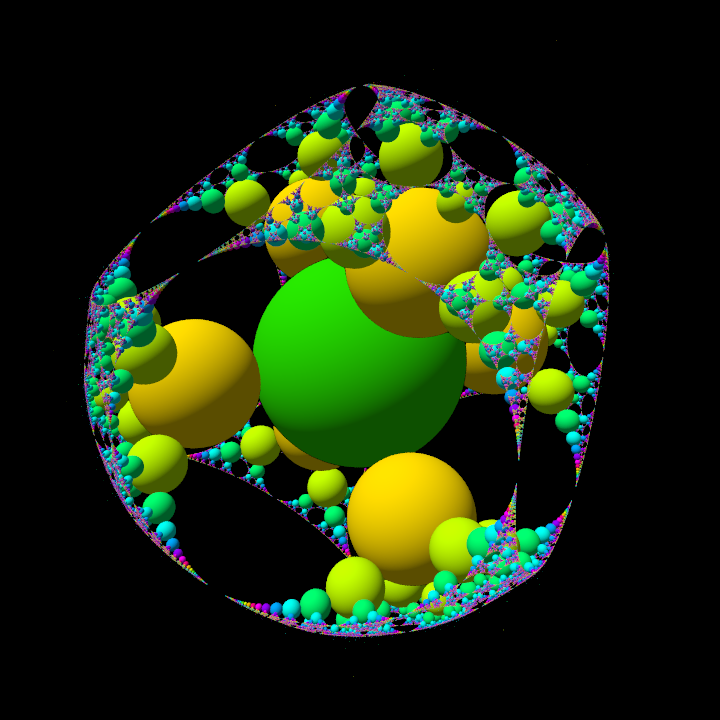
\includegraphics[height=1.35in, keepaspectratio]{img/preparation/3dExtension/3dOrbit.png}
  \caption{\textit{The orbit of the green sphere}}
  \label{fig:orbitCat}
  \hspace*{\fill}
 \end{minipage}
\end{figure}

We use \textit{Sphere Tracing} to render three dimensional
fractals and orbit of the seed sphere.
Sphere Tracing is one of the algorithm to ray tracing.

\subsection{Related Works}

Aaron Montag uses texture based approach to visualize limit set of the
Kleinian groups \cite{Montag2014hyperbolicIFS}.
%% テクスチャベースの描画方法 テクスチャに種となる円を描き,円に変換を作
%% 用させることで極限集合を描画させる

Jos Leys invented efficient algorithm to draw Kleinian group with Maskit
parametrization. IIS uses circle inversions on the other hand Jos Leys
uses normal generators.
%% IISを普通の関数を使って行っている こちらのIISは円,球に注目している

Martin von Gagern introduce similar algorithm called \textit{Reverse
Pixel Lookup} \cite{journals/combinatorics/GagernR09}. The algorithm is for visualizing tiling.